\section{Pull-back convexity}\label{convexity}

The part \ref{thm:convexity:convexity} of Theorem~\ref{thm:convexity} follows from the three propositions in this section.

\begin{thm}{Proposition}\label{prop:CTIL}
If a complete Riemannian manifold satisfies 4(1)-tree comparison the it is CTIL.
\end{thm}

\parit{Proof.}
Assume that a Riemannian manifold $M$ satisfies 4(1)-tree comparison.
Assume there is $p\in M$ and $u,v\zz\in \TIL_p$ such that $w=\tfrac12\cdot(u+v)\notin \TIL_p$.
It is sufficient to show that $\gamma(t)=\exp_p(w\cdot t)$ is a length-minimizing on $[0,1]$.

Assume the contrary, that is, $\tau<1$ is the maximal value such that the geodesic $\gamma(t)=\exp_p(w\cdot t)$ is a length-minimizing on $[0,\tau]$.
Set $w'=\tau\cdot w$.
Note that $w'\in\partial \TIL_p$.


Set $q=\exp_p w'$.
By general position argument, we can assume that there are at least two minimizing geodesics connecting $p$ to $q$; see \cite{karcher}.
That is, there is $w''\in \partial \TIL_p$ such that 
$w''\ne w'$
and $\exp_pw'=\exp_pw''$.

\begin{center}
\begin{lpic}[t(-0 mm),b(-0 mm),r(0 mm),l(0 mm)]{pics/7-config(1)}
\lbl[r]{1.5,32;$x$}
\lbl[l]{59.5,31;$y$}
\lbl[t]{18.5,2;$y'$}
\lbl[t]{32.5,2;$x'$}
\lbl[t]{26,4.5;$p$}
\lbl[r]{23,14;$z$}
\lbl[b]{28,31;$q$}
\lbl[l]{30,23;$q'$}
\end{lpic}
\end{center}

Fix small small positive real numbers $\delta,\eps$ and $\zeta$.
Consider the following points
\begin{align*}
q'=q'(\eps)&=\exp_p(1-\eps)\cdot w',
&
z=z(\zeta)&=\exp_p(\zeta\cdot w''),
\\
x&=\exp_p u,
&
x'=x'(\delta)&=\exp_p (-\delta\cdot u),
\\
y&=\exp_p v,
&
y'=y'(\delta)&=\exp_p (-\delta\cdot v).
\end{align*}

We will  show that for some choice of $\delta,\eps$ and $\zeta$ the tree comparison for $p/xx'yy'(q'/z)$ does not hold.

Assume the contrary, that is, given any positive numbers $\delta,\eps$ and $\zeta$, there is a point array $\~p$, $\~x$, $\~x'(\delta)$, $\~y$, $\~y'(\delta)$, $\~q'(\eps)$, $\~z(\zeta)\in\HH$ as in the definition of $T$-tree comparison.

\begin{wrapfigure}{r}{35 mm}
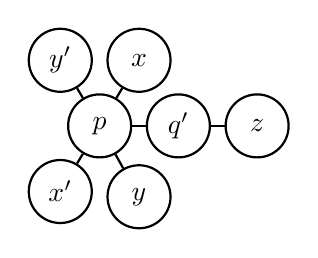
\begin{tikzpicture}[scale=1,
  thick,main node/.style={circle,draw,font=\sffamily\bfseries,minimum size=8mm}]

  \node[main node] (0) at (3/2,11/6){$x$};
   \node[main node] (1) at (1/2,1/6){$x'$};
  \node[main node] (2) at (3/2,.1){$y$};
  \node[main node] (3) at (1,1){$p$};
  \node[main node] (4) at (1/2,11/6){$y'$};
  \node[main node] (5) at (3,1){$z$};
  \node[main node] (6) at (2,1){$q'$};

  \path[every node/.style={font=\sffamily\small}]
     (0) edge node[above]{}(3)
   (1) edge node[above]{}(3)
   (2) edge node[above]{}(3)
   (3) edge node[above]{}(6)
   (4) edge node[above]{}(3)
   (5) edge node[above]{}(6);
\end{tikzpicture}
\end{wrapfigure}

If $\delta$ is small, we can assume that $p$ lies on a necessary unique minimizing geodesic $[x\,x']_M$.
Hence 
\[|x-x'|_M=|x-p|_M+|p-x'|_M.\]
By comparison
\begin{align*}
|\~x-\~x'|_\HH&\ge|x-x'|_M,
\\
|\~x-\~p|_\HH&=|x-p|_M,
\\
|\~x'-\~p|_\HH&=|x'-p|_M.
\end{align*}
By triangle inequality,
\[|\~x-\~x'|_\HH=|\~x-\~p|_\HH+|\~x'-\~p|_\HH;\]
that is, $\~p\in [\~x\,\~x']_\HH$.
The same way we see that $\~p\in [\~y\,\~y']_\HH$.

Fix $\eps$ and $\zeta$.
Note that as $\delta\to 0$ we have 
\begin{align*}
\~x'&\to \~p,
&
\~y'&\to \~p.
\\
\measuredangle[\~p\,^{\~x'}_{\~y}]&\to \measuredangle[p\,^{x'}_{y}],
&
\measuredangle[\~p\,^{\~y'}_{\~x}]&\to \measuredangle[p\,^{y'}_{x}],
\\
\measuredangle[\~p\,^{\~x'}_{\~q'}]&\to \measuredangle[p\,^{x'}_{q'}],
&
\measuredangle[\~p\,^{\~y'}_{\~q'}]&\to \measuredangle[p\,^{y'}_{q'}],
\end{align*}
It follows that 
\begin{align*}
\measuredangle[\~p\,^{\~x}_{\~y}]&\to \measuredangle[p\,^x_y],
&
\measuredangle[\~p\,^{\~x}_{\~q'}]&\to \measuredangle[p\,^x_{q'}],
&
\measuredangle[\~p\,^{\~y}_{\~q'}]&\to \measuredangle[p\,^y_{q'}].
\end{align*}


Therefore, passing to a partial limit as $\delta\to0$, we get a configuration of 5 points 
$\~p, \~x,\~y,\~q'=\~q'(\eps),\~z=\~z(\zeta)$ such that  
\begin{align*}
\measuredangle[\~p\,^{\~x}_{\~y}]&= \measuredangle[p\,^{x}_{y}],
&
\measuredangle[\~p\,^{\~y}_{\~q'}]&= \measuredangle[p\,^{y}_{q'}],
&
\measuredangle[\~p\,^{\~x}_{\~q'}]&= \measuredangle[p\,^{x}_{q'}].
\end{align*}
In other words, the map sending the points $0,u,v,w'\in\T_p$ to $\~p,\~x,\~y,\~q\in\HH$ correspondingly is distance preserving.

Note that $q'\to q$ as $\eps\to0$. 
Therefore, in the limit,
we get a configuration $\~p$, $\~x$, $\~y$, $\~q'$, $\~z=\~z(\zeta)$ such that in addition we have
\begin{align*}
|\~q'-\~z|&=|q-z|,
&
|\~p-\~z|&\ge |p-z|,
\\
|\~x-\~z|&\ge |x-p|,
&
|\~y-\~z|&\ge |y-z|
\end{align*}

Since $w''\ne w'$, for small values $\zeta$ the last three inequalities 
imply 
\[|\~q'-\~z|>|q-z|,\]
a contradiction.

\begin{thm}{Proposition}\label{prop:convex}
If  a complete CTIL Riemannian manifold $M$ satisfies 4(1)-tree comparison,
then for any $p,q\in M$, we have $f''\le 1$, where $f$ is the function $f\: \TIL_p\to \RR$ defined by
\[f(v)=\tfrac12\cdot\dist_q^2\circ\exp_p(v).\]

\end{thm}

\parit{Proof.}
Note that 4(1)-tree comparison implies 3-tree comparison.
Hence $M$ has nonnegative sectional curvature.

Fix $u,v\in \TIL_p$ and $w\in [u\,v]$.
It is sufficient to show that there is a function $g\:\T_p\to \RR$ such that
\[g''=1,\quad
g(w)=f(w),\quad
g(u)\ge f(u)\quad
\text{and}\quad
g(v)\ge f(v).\]

Fix small $\eps>0$ and set
\begin{align*}
x&=\exp_p u,
&y&=\exp_p v, 
&z&=\exp_pw,
\\
x'&=\exp_p(-\eps\cdot  u),
&y'&=\exp_p(-\eps\cdot  v).
\end{align*}
Apply the $p/xyx'y'(z/q)$ comparison and pass to the limit as $\eps\to 0$.
We obtain a configuration of points $\~p, \~x, \~y, \~z, \~q\in\HH$, satisfying corresponding comparisons and
in addition
\begin{align*}
\measuredangle[\~p\,^{\~x}_{\~y}]&= \measuredangle[p\,^{x}_{y}],
&\measuredangle[\~p\,^{\~x}_{\~z}]&= \measuredangle[p\,^{x}_{z}],
&\measuredangle[\~p\,^{\~z}_{\~y}]&= \measuredangle[p\,^{z}_{y}].
\end{align*}
In particular,
from above and Toponogov comparison, we have
\begin{align*}
|\~x-\~y|_\HH&=|u-v|_{\T_p},
&|\~z-\~y|_\HH&=|w-v|_{\T_p},
&|\~x-\~z|_\HH&=|u-w|_{\T_p},
\\
|\~q-\~z|_\HH&=|q-z|_M,
&|\~q-\~x|_\HH&\ge|q-x|_M,
&|\~q-\~y|_\HH&\ge|q-y|_M.
\end{align*}
In particular, there is a distance-preserving map $\T_p\to \HH$ 
such that $u\mapsto \~x$, $v\mapsto \~y$, $w\mapsto \~z$ and $0\mapsto \~p$.
Further, we identify $\T_p$ and a subset of $\HH$ using this map.

Consider the function $g(s):=\tfrac12\cdot|s-\~q|_{\T_p}^2$.
Note that $g''=1$ and
\begin{align*}
g(w)&=\tfrac12\cdot|\~q-\~z|_{\T_p}^2
=\tfrac12\cdot|q-z|_M^2
=f(w),
\\
g(u)&=\tfrac12\cdot|\~q-\~x|_{\T_p}^2
\ge \tfrac12\cdot|q-x|_M^2
=f(u),
\\
g(v)&=\tfrac12\cdot|\~q-\~y|_{\T_p}^2
\ge\tfrac12\cdot|q-y|_M^2
= f(u).
\end{align*}
Hence the first statement follows.

\begin{thm}{Proposition}\label{prop:m(n)}
Assume $M$ is a complete CTIL Riemannian manifold such that for any $p,q\in M$, we have $f''\le 1$, where $f$ is the function $f\: \TIL_p\to \RR$ defined by
\[f(v)=\tfrac12\cdot\dist_q^2\circ\exp_p(v),\]
Then $M$ satisfies all bipolar tree comparisons.
\end{thm}

\parit{Proof.}
Fix points $p$ and $q$ in $M$;
set $\~q=\log_pq\in\T_p$ and $\~f(v)=\tfrac12\cdot |v-\~q|_{\T_p}^2$.
Note that 
\[f\le \~f.\eqlbl{eq:f=<f}\]
Further note that the inequality \ref{eq:f=<f} is equivalent to the Toponogov comparison for all hinges $[p\,{}^x_q]$ in $M$.
It follows that $M$ has nonnegative sectional curvature. 

\medskip

Fix a bipolar geodesic tree $[p/x_1\dots x_n(q/y_1\dots y_m)]$ in $M$.
Set 
\[\~p=0=\log_pp,\quad \~q=\log_pq,\quad\text{and}\quad \~x_i=\log_px_i\]
for each $i$. 

Consider the linear map $\psi_1\:\T_q\to \T_p$ such that for any smooth function $h$
\[\psi_1\:\nabla_{q}h\mapsto \nabla_{\~q}(h\circ\exp_p).\]
Since sectional curvature of $M$ is nonnegative, the restriction $\exp_p|_{\TIL_p}$ is short and therefore so is $\psi_1$.

In particular there is a linear map $\psi_2\:\T_q\to\T_p$ such that, the map $\iota\:\T_q\zz\to \T_p\oplus\T_p$ defined by
\[\iota\:v\mapsto \psi_1(v)\oplus \psi_2(v)\]
is distance preserving.

Further set 
\[h_i=\tfrac12\cdot\dist_{y_i}^2,
\quad
g_i=h_i\circ\exp_p|_{\TIL_p},
\quad
\~y_i=\~q-\iota(\nabla_q h_i).
\]


By construction
\[|\~y_i-\~q|_{\T_p\oplus\T_p}=|y_i-q|_M.\]

At the point $\~q$ the restriction functions $\~g_i=\tfrac12\cdot\dist^2_{\~y_i}|_{\T_p\oplus 0}$ and the function $g_i$ have the same value and gradient.
Since $g_i''\le 1$ and $\~g_i''=1$, we get $\~g_i\ge g_i$. 
The latter implies
\[
|\~y_i-\~p|_{\T_p\oplus\T_p}\ge|y_i-p|_M
\quad
\text{and}
\quad
|\~y_i-\~x_j|_{\T_p\oplus\T_p}\ge|y_i-x_j|_M.\]
for any $i$ and $j$.

Since there is an isometric embedding $\T_p\oplus\T_p\hookrightarrow \HH$,
we get the needed configuration.
\qeds


